% !TeX root = ../../tesi.tex

For the computations at Site~2, namely RGB image acquisition, local control of the sensing pipeline, and execution of lightweight edge-processing tasks, the \textbf{Raspberry Pi 5} was adopted.\cite{raspberrypi_raspberry_pi_5_2026} In contrast to Site~1, where an RGB-D sensor and an embedded GPU platform were required for volumetric estimation, Site~2 relies on a monocular RGB setup and therefore benefits from a more compact and cost-effective embedded computer.

\begin{figure}[h]
    \centering
    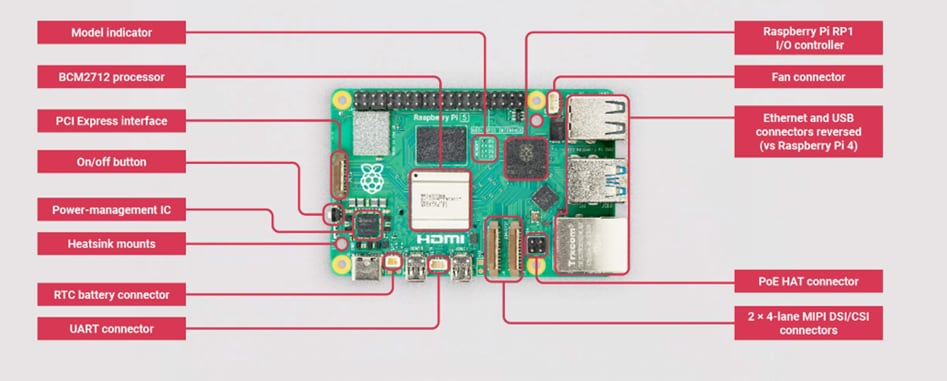
\includegraphics[width=0.7\textwidth]{images/Raspberry.jpg}
    \caption{Raspberry Pi 5 board.}
    \label{fig:rpi5_board}
\end{figure}

The Raspberry Pi 5 is a single-board computer developed for embedded and edge-computing applications.\cite{raspberrypi_raspberry_pi_5_2026} It is based on the Broadcom BCM2712 system-on-chip, which integrates a \textbf{quad-core Arm Cortex-A76 CPU running at 2.4~GHz}, a \textbf{VideoCore~VII GPU}, and \textbf{8~GB of LPDDR4X memory} in the configuration adopted for this project.\cite{raspberrypi_raspberry_pi_5_2026}

From a hardware standpoint, the Raspberry Pi 5 provides a wide set of interfaces that are particularly relevant for computer-vision deployments, including:
\begin{itemize}
    \item two USB~3.0 ports and two USB~2.0 ports,
    \item Gigabit Ethernet,
    \item dual-band Wi-Fi and Bluetooth connectivity,
    \item two four-lane MIPI transceivers for camera and display interfaces,
    \item a PCIe~2.0 interface for high-speed peripheral expansion,
    \item a USB-C power input.\cite{raspberrypi_raspberry_pi_5_2026}
\end{itemize}

These characteristics make the platform flexible enough to support local image acquisition, communication with external devices, and integration with dedicated sensing peripherals such as the Raspberry Pi Camera Module~3 Wide discussed in the following subsection.\cite{raspberrypi_raspberry_pi_hardware_2026}

An important practical aspect of the Raspberry Pi 5 is that its increased computing performance, compared with earlier Raspberry Pi boards, is accompanied by a higher thermal load under sustained workloads. Since the device in the present application is expected to operate continuously for long periods, potentially day and night and without constant supervision, it is important to equip it with an active cooling system in order to reduce the risk of thermal throttling and to maintain stable performance under prolonged load.\cite{raspberrypi_raspberry_pi_5_2026} For this reason, the board was installed inside a protective case equipped with a fan, as shown in Figure~\ref{fig:rpi5_site2}.

\begin{figure}[h]
    \centering
    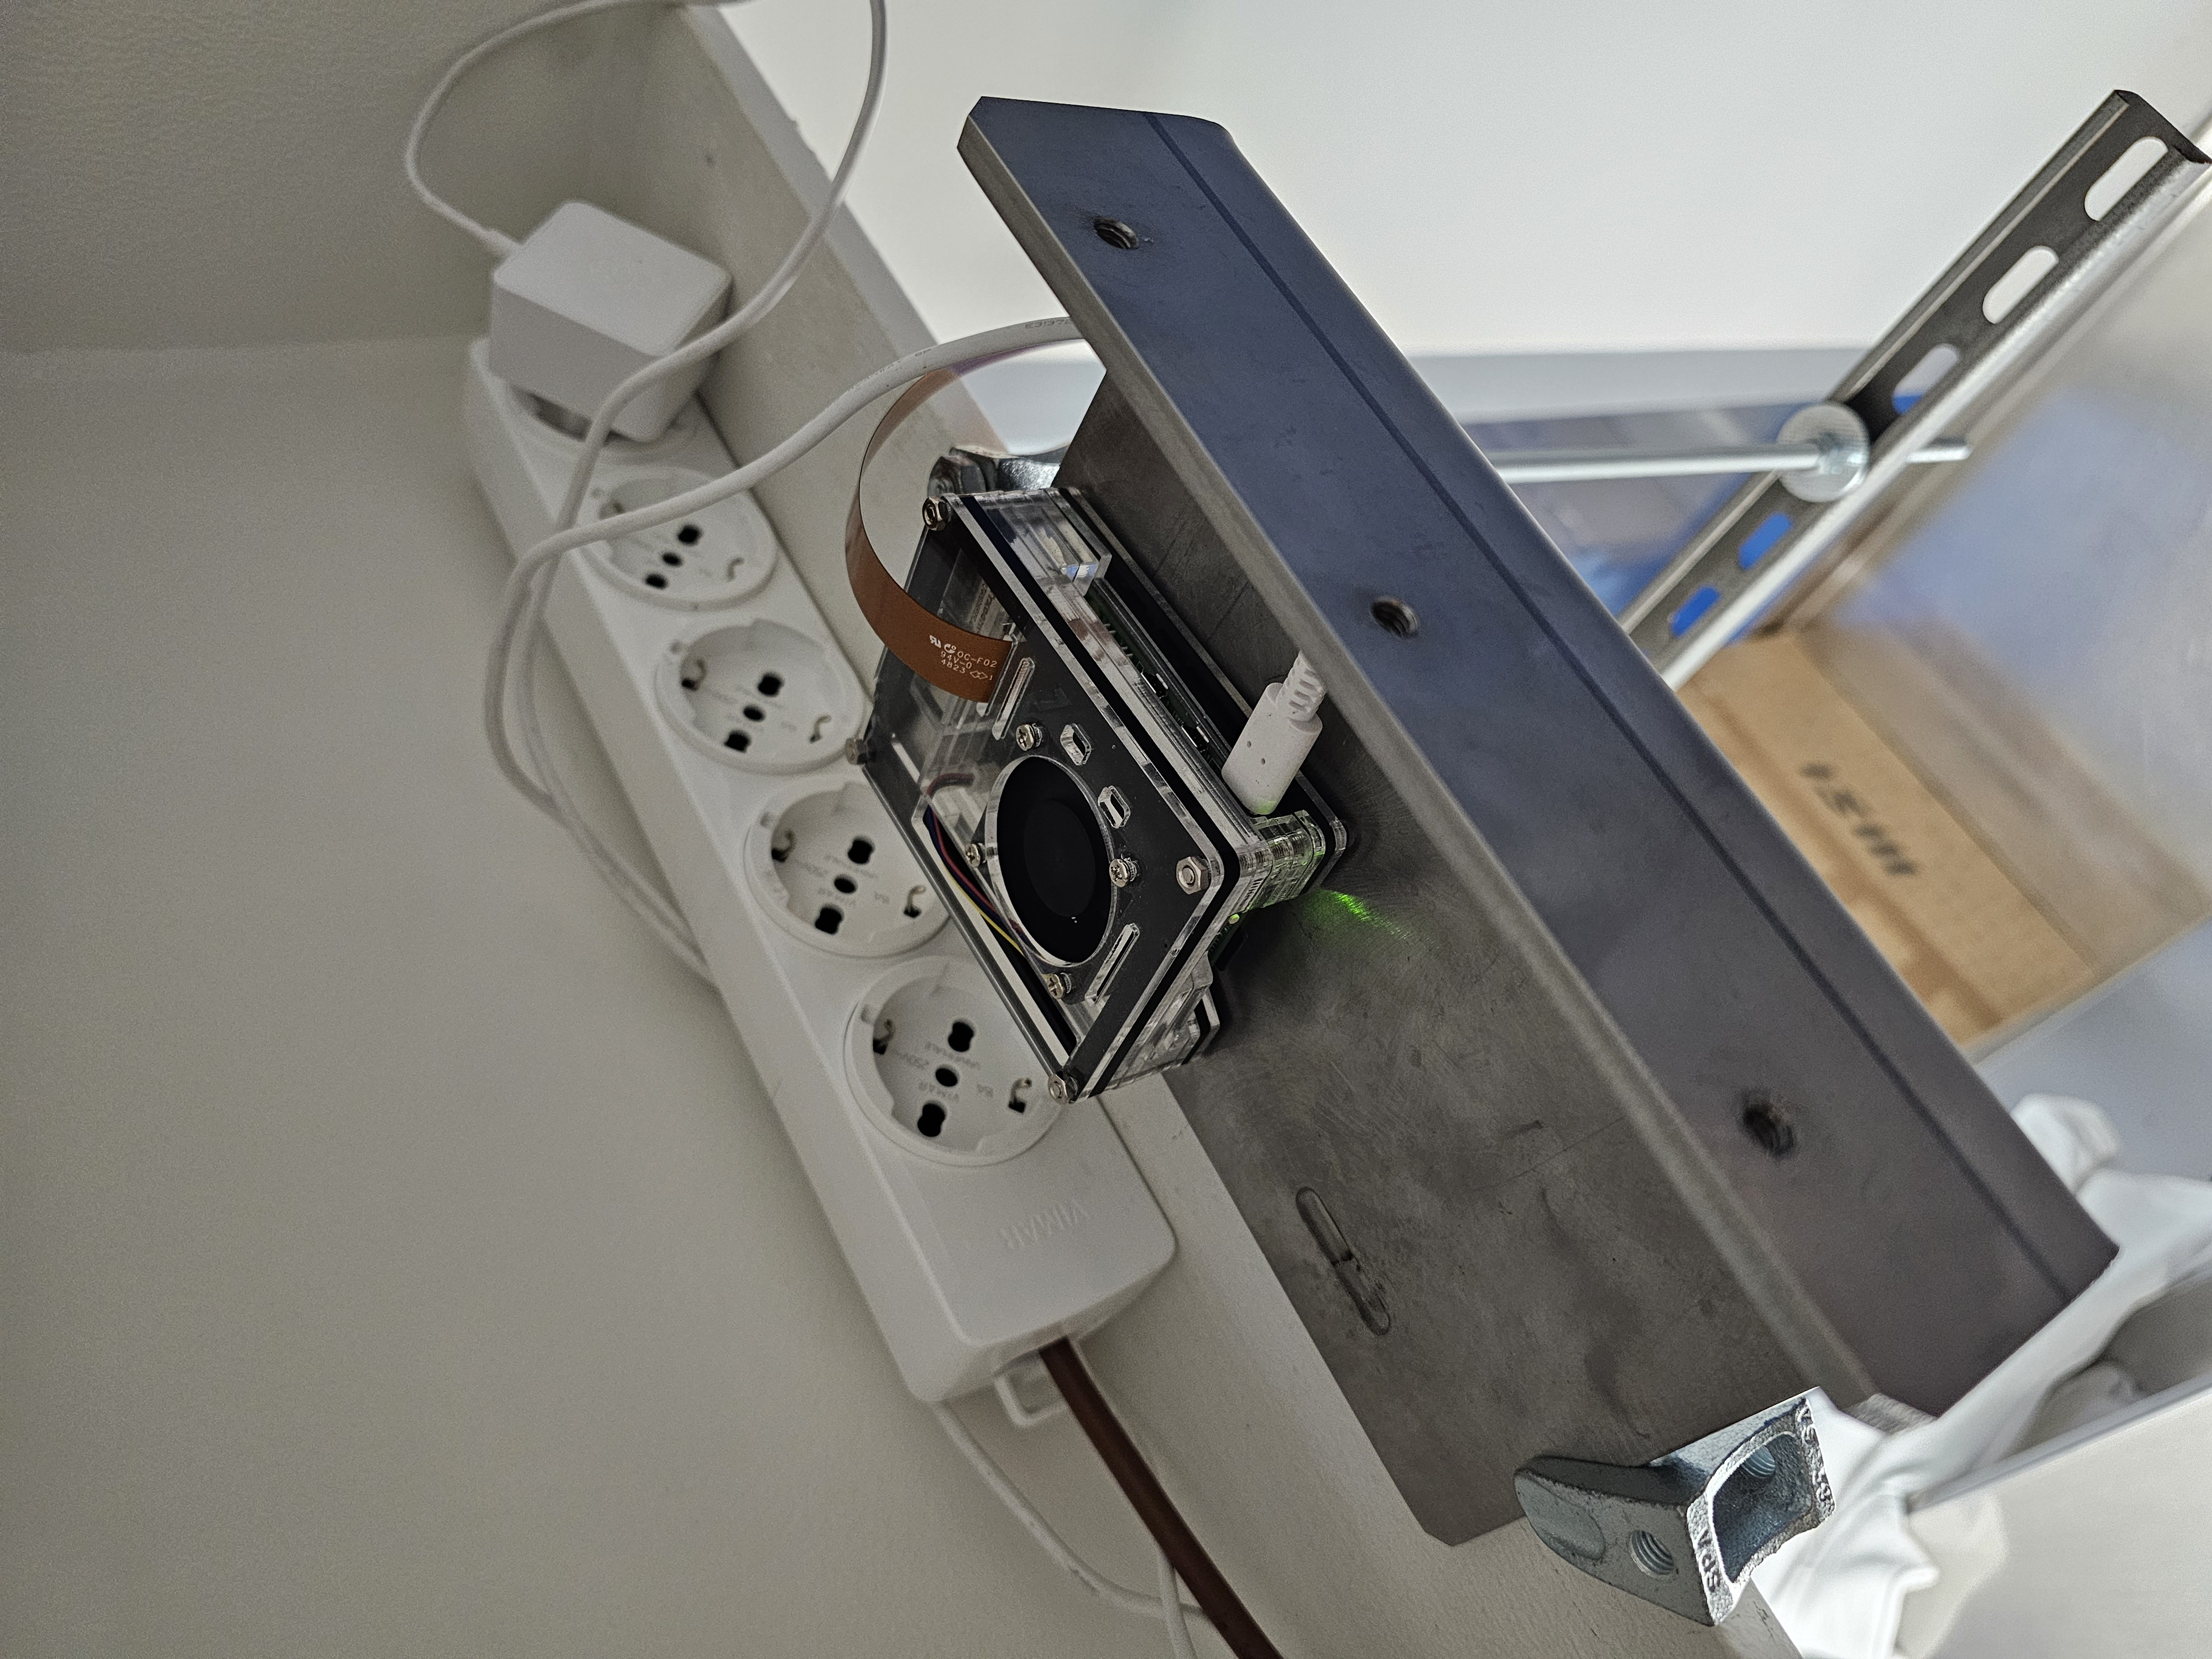
\includegraphics[width=0.6\textwidth, angle=-90]{images/Raspberry_sito2.jpg}
    \caption{Raspberry Pi 5 installed on Site~2 inside a protective case with active cooling.}
    \label{fig:rpi5_site2}
\end{figure}

From the perspective of the present application, the Raspberry Pi 5 offers several advantages: compact size, low power requirements, straightforward integration with official Raspberry Pi peripherals, and sufficient computational capability for a lightweight vision pipeline at the edge. At the same time, compared with more specialized embedded AI platforms such as the Jetson Nano, it provides a less dedicated acceleration stack for deep-learning inference. In this sense, its adoption at Site~2 is justified by the lower sensing complexity of the setup, which is based only on RGB imagery and does not require real-time RGB-D reconstruction or point-cloud processing. Considering the trade-off between computational capability, ease of integration, cost, and deployment simplicity, the Raspberry Pi 5 represents a suitable hardware platform for Site~2.\cite{raspberrypi_raspberry_pi_5_2026,raspberrypi_raspberry_pi_hardware_2026}
